\documentclass[preprint]{elsarticle}
\usepackage[utf8]{inputenc}
\usepackage{amsmath}
\usepackage{amsfonts}
\usepackage{tikz}
\usetikzlibrary{shapes.misc,shadows}
\usetikzlibrary{positioning} 
\usepackage{amsthm}
\usepackage{array}
\usepackage{parskip}
\usepackage{float}
\usepackage{paralist}
\usepackage{listings}
\usepackage{color}
\usepackage{caption}
\usepackage{tablefootnote}
\usepackage{hyperref}
\usepackage{multirow}
\usepackage[cache=false,section]{minted}
\usepackage[a4paper, total={6in, 8in}]{geometry}
\usepackage[tworuled,algosection,figure,linesnumbered]{algorithm2e}
\usepackage{glossaries}
\usemintedstyle{default}
\newminted{haskell}{frame=lines,framerule=2pt}
\newminted{R}{frame=lines,framerule=2pt}
\graphicspath{{./images/}}

\bibliographystyle{abbrvnat}

\makeglossaries

\newacronym{dp}{DP}{Dynamic Pipeline Paradigm}
\newacronym{bfs}{BFS}{Breadth-First Search}
\newacronym{dfs}{DFS}{Depth-First Search}
\newacronym{wcc}{WCC}{Weak Connected Components}
\newacronym{haskell}{Haskell}{Haskell Programming Language}
\newacronym{fp}{FP}{Functional Programming}
\newacronym{rl}{R}{R Language}
\newacronym{os}{OS}{Operative System}


\newtheorem{thm}{Theorem}
\newtheorem{lem}[thm]{Lemma}
\newdefinition{prob}{Problem}
\newdefinition{defin}{Definition}
\newdefinition{rmk}{Remark}
\newproof{pf}{Proof}
\newproof{pot}{Proof of Theorem \autoref{thm2}}

%\title{Towards a Haskell Abstraction of Dynamic Pipeline %Paradigm\tnoteref{t1}}

\title{Towards a Dynamic Pipeline Framework implemented in (parallel) Haskell\tnoteref{t1}}

\tnotetext[t1]{This work has been partially supported by funds from the Spanish Ministry for Science and Innovation and the European Union (FEDER funds) under grant MOTION (ref. TINXXXXXXXX)}
%
\author[1]{Juan Pablo Royo Sales}
\ead{juan.pablo.royo@estudiantat.upc.edu}

\author[1]{Edelmira Pasarella}
\ead{edelmira@cs.upc.edu}

\author[1]{Cristina Zoltan}
\ead{zoltan@cs.upc.edu}

\author[2]{Maria-Esther Vidal}
\ead{maria.vidal@tib.eu}

\affiliation[1]{organization={Universitat Politecnica de Catalunya},
postcode={08034},
city={Barcelona},
country={Spain}}

\affiliation[2]{organization={TIB/L3S Research Centre at the University of Hannover},
%addressline={JWRA 34, Jagathy},
%postcode={695014},
city={Hannover},
country={Germany}}

\begin{document}

\begin{abstract}
Data streaming processing has giving rise to new computation paradigms to provide effective and efficient processing of data streams. The most important features of these new paradigms is the exploitation of  the parallelism, the capacity of adapting execution schedulers, reconfigure computational structures, adjust the use of resources according to the characteristics of the input stream and produce incremental results. The Dynamic Pipeline Paradigm is a naturally functional approach to deal with stream processing. This fact encourages us to use a  pure functional programming language to implement a Dynamic Pipeline Framework (DPF).  In this work we tackled the problem of assessing the suitability of using (parallel) Haskell to implement a DPF.  The justification of this choice is twofold: From a formal point of view, Haskell has strong theoretical foundations providing the possibility of manipulating computations as primary entities and, from a practical point of view,  it has a powerful set of tools for writing multithreading and parallel computations with optimal performance. Firstly, we conduct an empirical evaluation to assess the performance of an \textit{ad-hoc} Haskell implementation of a naive dynamic pipeline to compute  the weak connected components of a graph (WCC).  After analyzing the results of the empirical evaluation we obtained insights on  the basis to construct parallel solutions using the Dynamic Pipeline Paradigm and the more relevant  factors that impact its scalability.  This allowed us to isolate which are the Haskell abstractions to be redefined and which new ones must be defined as well as the systems parameters to be considered to lift the WCC dynamic pipeline to a general  DPF implementation. Finally, we present a first approach of a general parametric DPF implementation.

%\textit{\acrfull{dp}} has been defined in order to solve problems where the data is heterogeneous 
%and in motion. Taking advantage on pipelining stage parallelization, this paradigm allows to dynamically adapt 
%stage computations according to the input. It has been shown in the definition of this computational model that any
%implementation attempt of the paradigm requires fast and flexible parallelization techniques as well as tools that 
%are suitable with the notion of computation as a \emph{first-class citizen}. In this work, we implement the \textit{Dynamic Pipeline Paradigm}
%in \texttt{Haskell} for solving the problem of finding \textit{Connected Components of a Graph}. We experiment with different kind of Graphs and show how %\texttt{Haskell} behaves on that context. Through this approximation we generate enough evidence to support that \texttt{Haskell} it is a suitable Language %for implementing \textit{Dynamic Pipeline Paradigm} not only because of its strong theoretical foundations which provides different Abstraction to manipulate %computations as primary entities with Mathematical reasoning, but also because it has a powerful Set of Tools for writing multithreading and parallel %computations.
\end{abstract}

\begin{keyword}
Dynamic pipeline \sep Haskell \sep parallelism \sep concurrency
\end{keyword}

\maketitle

\section{Introduction}
Traditionally, \acrfull{haskell} has been considered as an academic language instead of a production language. However it is lastly well known that in addition to its strong theoretical foundations it has a powerful set of tools for writing multithreading and parallel programs with optimal performance.

On the other hand, \textit{\acrfull{dp}} \citep{dpdef} offers a promising model for Big Data Streaming Processing taking advantage of Pipeline Parallelization. 

One of the biggest challenge of \acrshort{dp} is to find a proper set of tools and programming language which can take advantage from both: \begin{inparaenum}[i\upshape)]
\item  \emph{fast parallel} processing and 
\item  \emph{strong theoretical} foundations that manage computations as first-class citizens.
 \end{inparaenum}

On this work, we conduct an implementation of \acrshort{dp} for solving \acrfull{wcc} with \acrshort{haskell} showing that both aspects mentioned can be covered with \acrshort{haskell}. At the same time we run some experiments to validate our assumptions about the feasibility of the chosen language, as well as providing a first approximation Design of a General Purpose \acrshort{dp} Library in \acrshort{haskell}.

\textbf{Problem Research and Objective:}\label{research:obj} Given the problem of \acrshort{wcc}, we explore the implementation of \acrshort{dp} using \acrshort{haskell} as a suitable Language for conducting this implementation. Working with this particular problem of \acrshort{wcc}, we explore the level of parallelism that \acrshort{haskell} offers and the speed improvement obtained as a result of that. As an additional goal, we define the first abstraction approximation  library or framework of \acrshort{dp} in \acrshort{haskell}.

\textbf{Approach:} In the first section of our work we present the \emph{Motivation Example} that is conducting this work (\acrshort{wcc}). Following that we define \acrshort{dp} Paradigm and at the same time we expose what are the premises that support \acrshort{haskell} as a suitable language for this implementation.
In the next part we are going to show the details of the Implementation that we have done in \acrshort{haskell} to solve the \emph{Motivating Example} proposed. In addition to that we present our \emph{Empirical Evaluation} which are going to answer our Hypothesis.
Finally we show the \emph{First Approximation} of the Design of a \emph{Dynamic Pipeline Framework} implemented in \acrshort{haskell}.

\textbf{Contributions:} Show \acrshort{haskell} is a suitable Language for implementing \acrshort{dp}, generating enough evidence through an Empirical Evaluation based on a Example problem (\acrshort{wcc}). This work also contribute in building the first abstraction approximation of \acrshort{dp} in \acrshort{haskell} as a future Framework/Library of this Computational Model in that Language. 


\section{Motivating Example}
We have selected \acrfull{wcc} as a motivational example problem for conducting this work. This has been already described in previous \acrshort{dp} work \citep{dpdef} as one of the suitable problems to be solve by this Paradigm.

\begin{defin}
A connected component of a graph $G$ is a connected subgraph $S$ of $G$ that is not a proper subgraph
of another connected subgraph $S'$ of $G$. Therefore, a connected component of a graph $G$ is a maximal
connected subgraph of $G$.
\end{defin}

Given an undirected graph $G = (V, E)$, we can find \acrshort{wcc} of $G$ in $O(V + E)$ using \textit{\acrfull{dfs}} or \textit{\acrfull{bfs}} algorithm \citep{CormenLeisersonEtAl09}. 

Although this problem can be solved in linear time, when we are manipulating real-world graphs, which are usually big, it would be better to have a computational model where this can be processed faster. \acrshort{dp} with its \textit{Parallelization Pipeline model} improve that speed up on Big Graphs for finding \acrshort{wcc}.

Although this example does not present many challenges at algorithmic level, we consider a proper problem to explore our assumptions because of the following:

\begin{itemize}
    \item It allows us to compare \acrshort{dp} implementation against default implementation with \acrshort{dfs} and explore the difference in execution time between both
    \item It allows us to describe a simple algorithm on \acrshort{dp} model without expending efforts of solving some complex algorithmic problem which is not the main objective of this work
    \item It allows us to validate the correcteness of the implementation with \acrshort{dp} because of the first statement.
\end{itemize}

\section{Preliminaries}\label{section:prelim}
\subsection{Dynamic Pipeline Paradigm}\label{sub:sec:dp:par}
%
Stream Programming has becomed very popular and there are several frameworks that support it  based on the model of pipelines, fork, and join operators Spark\footnote{https://spark.apache.org/}, Knime\footnote{https://www.knime.com/}, Hadoop\footnote{https://hadoop.apache.org/}, etc. Algorithmic solutions based on this frameworks consists in describing dependencies among pieces of sequential  code/actors. To our knowledge, very few frameworks have constructions that allow programmers to express a pipeline having a variable length during program execution. A \textit{Dynamic Pipeline  (DP)}  \cite{dpdef} is a data-driven one-dimensional and unidirectional chain of stages connected by means of channels synchronized by data availability. This computational structure stretches and shrinks depending on the spawning and the lifetime of its stages, respectively. Modeling an algorithmic solution as a DP corresponds to define a dynamic computational structure  in terms of four kind of stages:  \textit{Input},  \textit{Generator},  \textit{Output} and \textit{Filter} stages.  To be concrete, the parameterized actors (algorithms)  corresponding to the behavior of each of these stages must be defined as well as the number and the type of the I/O channels connecting them. Channels are unidirectional  according to the flow of the data. Before executing an algorithm deployed as a  DP, the initial configuration of the pipe must be stated. This is, an initial pipe composed of a chain of instantiated stages: \textit{Input},  \textit{Generator} and \textit{Output}. \autoref{fig:initialpipe} depicts the initial state of a DP.  As data are incoming  the \textit{Generator} stage spawns \textit{Filter} stage instances. \textit{Filters} contains the actor(s) that occur when solving a problem. \autoref{fig:activepipe} illustrates this case.
%

\begin{figure*}[htbp]
\begin{center}
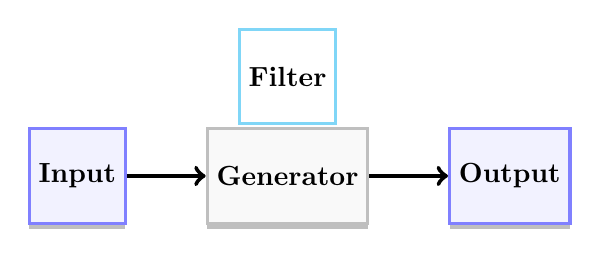
\begin{tikzpicture}[
ionode/.style={rectangle, draw=blue!50, fill=blue!5, very thick, minimum size=12mm, 
drop shadow={opacity=.5,shadow xshift=0pt},
},
gennode/.style={rectangle, draw=gray!50, fill=gray!5, very thick, minimum size=12mm, 
drop shadow={opacity=.5,shadow xshift=0pt},
},
filternode/.style={rectangle, draw=cyan!50, fill=white, very thick, minimum size=12mm, 
%drop shadow={opacity=.5,shadow xshift=0pt},
}]
%Nodes
\node[ionode]      (in)                              {\textit{\bf Input}};
\node[gennode]   (gen)                [right=of in] {\textit{\bf Generator}};
\node[ionode]      (out)                 [right=of gen] {\textit{\bf Output}};
\node[filternode]  (filter)                [above= 0.2mm of gen] {\textit{\bf Filter}};
%Lines
\draw[ultra thick,->] (in.east) -- (gen.west);
\draw[ultra thick,->] (gen.east) -- (out.west);
\end{tikzpicture}
\end{center}
\caption{{\bf Initial configuration of a Dynamic Pipeline.} 
Here the caption} 
\label{fig:initialpipe}
\end{figure*}
%
\begin{figure*}[htbp]
\begin{center}
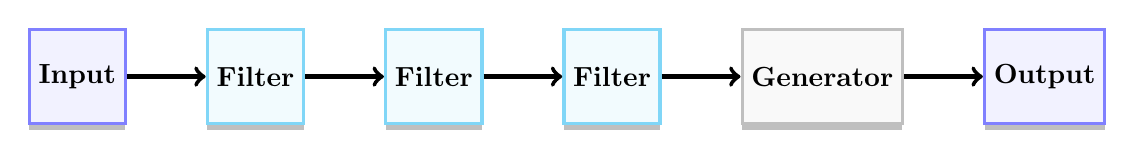
\begin{tikzpicture}[
ionode/.style={rectangle, draw=blue!50, fill=blue!5, very thick, minimum size=12mm, 
drop shadow={opacity=.5,shadow xshift=0pt},
},
gennode/.style={rectangle, draw=gray!50, fill=gray!5, very thick, minimum size=12mm, 
drop shadow={opacity=.5,shadow xshift=0pt},
},
filternode/.style={rectangle, draw=cyan!50, fill=cyan!5, very thick, minimum size=12mm, 
drop shadow={opacity=.5,shadow xshift=0pt},
}]
%Nodes
\node[ionode]      (in)                              {\textit{\bf Input}};
\node[filternode]  (filter1)               [right=of in] {\textit{\bf Filter}};
\node[filternode]  (filter2)               [right=of filter1] {\textit{\bf Filter}};
\node[filternode]  (filter3)               [right=of filter2] {\textit{\bf Filter}};
\node[gennode]   (gen)                 [right=of filter3] {\textit{\bf Generator}};
\node[ionode]      (out)                  [right=of gen] {\textit{\bf Output}};
\
%Lines
\draw[ultra thick,->] (in.east) -- (filter1.west);
\draw[ultra thick,->] (filter1.east) -- (filter2.west);
\draw[ultra thick,->] (filter2.east) -- (filter3.west);
\draw[ultra thick,->] (filter3.east) -- (gen.west);
\draw[ultra thick,->] (gen.east) -- (out.west);
\end{tikzpicture}
\end{center}
\caption{{\bf Dynamic Pipeline with some filter instances.} 
Here the caption}
\label{fig:activepipe}
\end{figure*}
%


\subsection{Haskell Implementation}\label{section:prob:dp:haskell}
Implementing a model of computation such as \acrshort{dp} requires certain characteristics that host Language and tools should provide in order to reach the desired objective. In regards to this, and according to what has been described on \autoref{section:prelim} we can argue that some of those primary aspects should be:

\begin{itemize}
    \item \textbf{Filters}: Since our Model is meant to generate dynamic computations (functions), throughout the Pipeline processing life cycle, our Language should be be able to have \textit{Functions} as a \textit{first-class citizens}
    \item \textbf{Dynamic Stages}: According to the previous item, it is not only require a strong representation of computation or functions but as well some Abstractions that can represent this dynamic behaviour which enlarge and shrink the pipeline but in terms of functions and not only data.
    \item \textbf{Parallelization}: Another key aspect on this model 
    \item \textbf{Channels}: Communication between Dynamic Stages, represented as \textit{Channels} by the Model, is the last key component.
\end{itemize}

Using a Language like \acrshort{haskell} fulfills completely all those requirements exposed before because of the following:

\begin{itemize}
    \item \textbf{Filters}: \acrfull{fp} Language like \acrshort{haskell} it is a perfect host for representing those \textit{Dynamic Computations}, not only due to its \acrshort{fp} nature, but also for it is Strong Type System which ensure safeness on the data representation pipeline and the computational sequence.
    \item \textbf{Dynamic Stages}\label{dyn:stage}: Abstractions like \textbf{Recursive Schemes} \citep{lenses} has been deeply explored and used in \acrshort{haskell} and allow us to represent in a formal and simple way \textit{dynamic} structure through \textit{Anamorphisms} and \textit{Catamorphisms}.
    \item \textbf{Parallelization}: Parallelization tehcniques and tools have also been intensively studied and implemented¡ in \acrshort{haskell} \citep{monadpar} and it is well known that \acrshort{haskell} light threads and spark allows to spawn thousands to millions of parallel computations without penalizing performance compare with \acrfull{os} level threading \citep{parallelbook}.
    \item \textbf{Channels}: As the last topic we have several techniques to our disposal to communicate between \textit{threads/sparks} in \acrshort{haskell} like \mintinline{haskell}{MVar} or concurrent safe like \mintinline{haskell}{STM}. Moreover we have at our disposal \textit{Channels} abstractions based on both mentioned communication mechanisms. 
\end{itemize}

Having exposing that, those are the reason that we believe \acrshort{haskell} is a perfect match for implementing \acrshort{dp} Paradigm\footnote{All the Source Code of this work can be found here https://github.com/jproyo/upc-miri-tfm/tree/feature/library-v1/connected-comp}.

\subsubsection{\textbf{Libraries and Tools}}\label{sub:lib:tools}
In this part we show how is the abstraction approximation that we design to represent \acrshort{dp} model in \acrshort{haskell}, but before showing the details it would be beneficial in order to understand the solution, to describe which libraries and tools have been decided to use.

As we have discussed before on \autoref{section:prob:dp:haskell}, there are at least 4 \emph{important aspects} in \acrshort{dp} design implementation to be covered: \begin{inparaenum}[i\upshape)]
\item \emph{Filters}
\item \emph{Dynamic Stages}
\item \emph{Parallelization}
\item and \emph{Channels}
 \end{inparaenum}.

\textbf{\textit{Filters}}\label{sub:sec:filter}: As we have discuss previously this is provided for free by the already built in language abstraction and the \acrshort{fp} paradigm itself where Functions are primary computational entities. Therefore there is no need to select any other additional library rather than using \emph{Monads} \citep{monads} for reflecting the Chain of Computations and the dependency between those computations, since we are implementing a Pipeline. In that sense if we represent \acrshort{dp} model as a \emph{Monad} we are getting for free the guarantee of \emph{Monad Laws}, in in particular \emph{Associativity law} which state that $(m >>= f ) >>= g = m >>= (\lambda x.f x >>= g)$ \citep{monadlaws}.

\textbf{\textit{Dynamic Stages}}: As well as in the previous point on \autoref{sub:sec:filter}, this is another abstraction that is already provided in the base library through the use of \mintinline{haskell}{fold} and \mintinline{haskell}{unfold} combinators which are the equivalent of \emph{Catamorphism} and \emph{Anamorphism} respectively. In this first approximation, we have chosen the simplest abstraction but as we mentioned before on \autoref{dyn:stage}, we believe that if we implement in a future work a proper \emph{Recursive Scheme} we can benefit of other properties and laws that those \emph{Fix Point Algebra and CoAlgebra Structures} \citep{lenses} provides. 

\textbf{\textit{Parallelization}}: One of the most important components on the implementation is the selection of \emph{Concurrency Library} to support an intensive parallelization workload. A direct guess to achieve this could be to use \textit{monad-par} library based on this work \citep{monadpar}, but we have discarded it because the Parallelism it is needed to be achieved is at \emph{Thread level} and not at \emph{Spark level}, due to the nature of \acrshort{dp}, where Pipeline Parallelism and not Data Parallelism is structural processing mechanism. The next obvious choice is to use \mintinline{haskell}{forkIO :: IO () -> IO ThreadId} from \mintinline{bash}{base} library, but that would imply to handle all the threads lifecycle, terminations and errors programmatically without major combinators or abstractions to deal with it. Therefore, we choose \textbf{async}\footnote{https://hackage.haskell.org/package/async} 
library which allow us to spawn asynchronous computations \citep{parallelbook} on \acrshort{haskell} and at the same time provides usefull combinators to managing thread terminations and errors.

\textbf{\textit{Channels}}\label{section:channels}: Finally the use of \emph{Channels} as a communication mechanism between Dynamic Stages and Data flowing in \acrshort{dp} model are implemented using \textbf{unagi-chan}\footnote{https://hackage.haskell.org/package/unagi-chan} library which provides the following advanateges to our solution:

\begin{itemize}
  \item \mintinline{haskell}{MVar} Channel with \textbf{no} use of \mintinline{haskell}{STM}: This allows to avoid internal locking for concurrent access. In this case
  we can use this advantage because in \acrshort{dp} model, one specific \textit{Pipeline Stage} which is running in a separated thread can only access to its \textit{Inputs/Outputs} channels for \textit{Reading/Writing} accordingly 
  and those operations are not concurrently share by other Threads (\textit{Stages}) for the same Channels.  
  \item \textbf{Non-Blocking} Channels: This library contains blocking and non-blocking Channels for reading and this is a key aspect to gain performance and speed up on the implementation.
  \item Optimized for $x86$ Architectures with use of low-level \textit{fetch-and-add} instructions.
  \item $100x$ faster on Benchmarking compare with \mintinline{haskell}{STM} and default base \mintinline{haskell}{Chan} implementations.
\end{itemize}

\section{A Connected Component Dynamic Pipeline Implementation}

\subsection{\textbf{DP Haskell Principal Algorithm}}

The following is the principal algorithm which represents the \textit{Monadic} computational chain of \acrshort{dp} main three \textit{Stages}: \begin{inparaenum}[i\upshape)]
\item \emph{Input}
\item \emph{Generator}
\item \emph{Output}
 \end{inparaenum}.

\begin{listing}[H]
\begin{minted}[fontsize=\small,numbers=left,frame=lines,framerule=2pt,framesep=2mm,baselinestretch=1.2,highlightlines={3,12}]{haskell}

runParallelDP :: Handle -> IO ()
runParallelDP h = input h >>= generator >>= output

input :: Handle -> IO (DP.Stream Edge ConnectedComponents)
input h = fromInput h >>= (|>> parseEdges)

output :: ConnCompDP -> IO ()
output = DP.mapM (R.putStrLn . show)

fromInput :: Handle -> IO (DP.Stream ByteString ConnectedComponents)
fromInput h = DP.unfoldM (B.hGetLine h) (R.hIsEOF h)

parseEdges :: ByteString -> IO [Edge]
parseEdges = toEdge . decodeUtf8

\end{minted}
\caption{Main algorithm \acrshort{dp} for \acrshort{wcc}}
\label{src:haskell:1}
\end{listing}

It can be seen in the \textbf{line 3} that the implementation of \acrshort{dp} in \acrshort{haskell} matches almost identically to the formal definition of proposed paradigm model.

We can also appreciate in the \textbf{line 12} the use of the \mintinline{haskell}{unfoldM} which is described in the Abstraction \acrshort{haskell} Library on \autoref{sub:inter:impl}.

It is important to notice that the input is being read in \textbf{non-blocking} mode and by batches of bytes\footnote{In this particular case by line because of parsing conveniences} allowing the streaming computation processing the edges as long as it arrives to the \textit{Generator} or the first \textit{Filter} Stages.\footnote{The format of the input file for the case of this example is an \textbf{edgelist} format compatible with \emph{igraph R library} or similar https://igraph.org/r/doc/write\_graph.html}

\subsection{\textbf{DP Connected Components in Haskell}}
In this subsection we are going to describe how we have implemented \acrshort{wcc} algorithm in \acrshort{dp} model with \acrshort{haskell}. Once we have the main components and the abstraction setup we only need to define how the \mintinline{haskell}{generator} function needs to behave and what the \textbf{filters} internally needs to do to process arriving data. 

\textbf{Generator:}\newline
The \textit{Generator} is the Computation in the Pipeline which is responsible to know when to interpose a new \textit{Filter} in front of the Pipe on \autoref{sub:sec:dp:par}.
In the case of \acrshort{wcc} a new \textit{Filter} is created on each new Edge that arrives to the \textit{Generator}.

\begin{listing}[H]
\begin{minted}[fontsize=\small,numbers=left,frame=lines,framerule=2pt,framesep=2mm,baselinestretch=1.2,highlightlines={2,11}]{haskell}
generator :: ConnCompDP -> IO ConnCompDP
generator = DP.foldrS createNewFilter
  where
    createNewFilter c v = do
      newInput  <- newChan
      newOutput <- newChan
      DP.Stream newInput newOutput 
            <$> async (newFilter (toConnectedComp v) c newInput newOutput)
  
  \end{minted}
  \caption{Generator \acrshort{dp} for \acrshort{wcc}}
  \label{src:haskell:2}
\end{listing}

As we can appreciate here, the highlighted \textbf{line 2} shows the use of the \acrshort{haskell} \textit{Catamorphism} which it is reducing the \textit{Stream} and at the same time creating the intermediate \textit{Filters} (Stages) of the Pipe.

\textbf{Filters:}\newline
In this case the algorithm is not as succinct as the previous because here is where the 2-step calculation takes place. As we have explained before each \textit{Filter} contains 2 sequential computations which are called \mintinline{haskell}{actor1} and \mintinline{haskell}{actor2}. The first one is responsible for gathering Connected Components based on the first Edge this \textit{Filter} was created from, and the second \textit{Actor} is responsible for \textit{combining} its own calculated Connected Components with others that are coming from the downstream. Representing sequential computations in \acrshort{haskell} is simple with \emph{Monadic} computations, which in this case \mintinline{haskell}{actor2} depends on the computation of \mintinline{haskell}{actor1}.

\begin{listing}[H]
\begin{minted}[fontsize=\small,numbers=left,frame=lines,framerule=2pt,framesep=2mm,baselinestretch=1.2,highlightlines={3,10-11,21-22}]{haskell}
newFilter :: ConnectedComponents -> ConnCompDP 
          -> DP.Channel Edge -> DP.Channel ConnectedComponents -> IO ()
newFilter conn inCh toInCh outCh = actor1 conn inCh toInCh >>= actor2 inCh toInCh outCh

actor1 :: ConnectedComponents -> ConnCompDP -> DP.Channel Edge -> IO ConnectedComponents
actor1 conn inCh toInCh = maybe finishActor doActor =<< DP.pullIn inCh
 where
  finishActor = DP.end' toInCh >> return conn

  doActor v | toConnectedComp v `intersect` conn = actor1 (toConnectedComp v <> conn) inCh toInCh
            | otherwise                          = v `DP.push'` toInCh >> actor1 conn inCh toInCh


actor2 :: ConnCompDP -> DP.Channel Edge 
       -> DP.Channel ConnectedComponents -> ConnectedComponents -> IO ()
actor2 inCh toInCh outCh conn = maybe finishActor doActor =<< DP.pullOut inCh

 where
  finishActor = conn `DP.push'` outCh >> DP.end' outCh

  doActor cc | conn `intersect` cc = actor2 inCh toInCh outCh (conn <> cc)
             | otherwise           = cc `DP.push'` outCh >> actor2 inCh toInCh outCh conn
\end{minted}
\caption{Filters \acrshort{dp} for \acrshort{wcc}}
\label{src:haskell:3}
\end{listing}

As we can see here, the algorithm for managing the Sets and do the \textit{Intersection} and \textit{Union} are not the  optimal for finding subgraphs\label{not:optimal}
\footnote{The propose of the present work is to present the implementation of \acrshort{dp} with \acrshort{haskell} but not working in the most optimal calculation of \acrshort{wcc}} and are base
on \mintinline{haskell}{Data.IntSet} module provided by \textbf{containers}\footnote{https://hackage.haskell.org/package/containers} library.

\section{Empirical Evaluation}
In the previous sections, we have described \acrshort{dp} Paradigm, our motivating example and why \acrshort{haskell} is a proper language for support that Model.
The empirical study aims at evaluating the performance of \acrshort{dp} when implemented in \acrshort{haskell}. 
Our goal is to answer the following research questions: 

\begin{enumerate}[Q1.]\label{res:question}
    \item Is \acrshort{haskell} going to support the dynamic parallelization level that \acrshort{dp} requires?\label{q:1}
    \item Is \acrshort{haskell} going to distribute and schedule the computations evenly among the processors and within them?\label{q:2}
    \item Is our implementation going to be at least $1.2$ faster compared with default implementations on base libraries for the same problem?\label{q:3}
    \item How the topology is affecting in the previous question and what are the particularities that \acrshort{dp} model should take into consideration for being faster?\label{q:4}
    \item Regarding memory allocation and management, is the implementation leaking memory or is it constant in memory space or even better than that?\label{q:5} 
\end{enumerate}

The following are the different kind of experiments we have conducted in order to test our assumptions and verify the correctness of the implementation.

\begin{itemize}
  \item \textbf{Real Graph Analysis}: In this case we have selected some Graphs from \textbf{Stanford Network Data Set Collection}\footnote{https://snap.stanford.edu/data/index.html} and analyze how the implementation
  behaves under bigger and real Graphs.
  \item \textbf{Benchmark}: Using \textit{criterion}\footnote{https://hackage.haskell.org/package/criterion} library, we have conducted a Benchmark between our solution and \acrshort{wcc} algorihtm under Base Haskell Library \mintinline{haskell}{Data.Graph}.
  \item \textbf{Performance Analysis}: Regarding performance analysis we have gather profiling data from \textit{GHC} for one of the Real Graph, in order to measure how the program performs on Multithreading execution and 
  on Memory Allocation.
\end{itemize}

\subsection{\textbf{Running Architecture}}

\begin{table}[H]
  \centering
  \begin{tabular}{|l|l|}
   \hline
   \textbf{Characteristic} & \textbf{Description} \\
   \hline
   Architecture & $x86$ $64$ bits  \\
   \hline
   Processor & $2,2$ GHz - $6$-Core Intel Core i7 up to $12$ Virtual cores \\
   \hline
   Hyper-Threading & Enable \\
   \hline
    L2 Cache & $256$ KB\\
    \hline
    L3 Cache & $9$ MB\\
    \hline
  \end{tabular}
 \caption{Experiments setup - Running Architecture}
 \label{run:arch}
 \end{table}

\subsection{\textbf{Haskell Setup}}

\begin{table}[H]
  \centering
  \begin{tabular}{|l|l|}
   \hline
   Compiler & \mintinline{bash}{GHC 8.10.4}  \\
   \hline
   \multirow{5}{5em}{Libraries} & \mintinline{bash}{async 2.2.3} \\ 
   & \mintinline{bash}{bytestring 0.10.12.0} \\
   & \mintinline{bash}{containers} 0.6.2.1 \\
   & \mintinline{bash}{relude 1.0.0.1} \\
   & \mintinline{bash}{unagi-chan 0.4.1.3}\\
   \hline
   \multirow{4}{7em}{Compilation Flags} & \mintinline{bash}{-threaded}\\
   & \mintinline{bash}{-O3}\\
   & \mintinline{bash}{-rtsopts}\\
   & \mintinline{bash}{-with-rtsopts=-N}\\
   \hline
  \end{tabular}
 \caption{Experiments setup - Haskell}
 \label{haskell:setup}
 \end{table}
 
\subsection{\textbf{DataSets}}\label{data:set}

For all the expirements we have been use the same Dataset taken from \textbf{Stanford Network Data Set Collection}\footnote{https://snap.stanford.edu/data/index.html}

\begin{table}[H]
  \centering
  \begin{tabular}{|p{0.25\linewidth}|r|r|r|r|r|}
   \hline
   \textbf{Network} & \textbf{Nodes} & \textbf{Edges} & \textbf{Mean Clust Coef} & \textbf{Diameter} & \textbf{\#\acrshort{wcc}}\\
   \hline
   Enron Emails \citep{netenron} & 36692 & 183831 & 0.4970 & 11 & 1065 \\
   \hline
   Astro Physics Collaboration Net \citep{netastro} & 18772 & 198110 & 0.6306 & 14 & 290\\
   \hline
   Google Web Graph \citep{netwebgoogle} & 875713 & 5105039 & 0.5143 & 21 & 2746\\
   \hline
  \end{tabular}
 \caption{DataSet of Graphs Selected}
 \label{table:4}
 \end{table}

\subsection{\textbf{Experiments Definition}}
\begin{table}[H]
  \centering
  \begin{tabular}{|l|p{0.15\linewidth}|p{0.2\linewidth}|p{0.2\linewidth}|p{0.2\linewidth}|l|}
   \hline
   \textbf{\#} & \textbf{Name} & \textbf{Goal} & \textbf{Motivation} & \textbf{How} & \textbf{Research Answer} \\
   \hline
   E1 & Graph Analysis & Measure GHC running time & Analyze execution time on Different Graph topologies & Enabling \mintinline{haskell}{+RTS -s} Flags & [Q4]  \\
   \hline
   E2 & Benchmark Analysis & Measure execution time over $4$ iterations for each Graph from the selected DataSet, both in the case of \texttt{DP} solution in \texttt{Haskell} and for the built-in base library of \texttt{Data.Graph} & Compare the solution with another implemented in the same language but with a different model & Use \emph{criterion}\tablefootnote{https://hackage.haskell.org/package/criterion} library  & [Q3,Q4] \\
   \hline
   E3 & Performance Analysis &Measure Internal Parallelism and Memory distribution of the solution & Verify empirically parallelization and memory behaviour of the program to see the feasibility of the implementation & Use \emph{ThreadScope}\tablefootnote{https://wiki.haskell.org/ThreadScope} for Threading analysis and \emph{eventlog2html}\tablefootnote{https://mpickering.github.io/eventlog2html/} for memory analysis & [Q1,Q2,Q5]\\
   \hline
  \end{tabular}
 \caption{Experiments setup - Definition}
 \label{table:exp:1}
 \end{table}


\section{\textbf{Discussion of Observed Results}}

\subsection{\textbf{Experiment: E1}}

The following represents the execution for running these graphs on our \acrshort{dp} implementation.

\begin{table}[H]
  \centering
  \begin{tabular}{|l|l|l|l|l|}
   \hline
   \textbf{Network} & \textbf{Exec Param} & \textbf{MUT Time} & \textbf{GC Time} & \textbf{Total Time}\\
   \hline
   Enron Emails & \mintinline{bash}{+RTS -N4 -s} & 2.797s & 0.942s & 3.746s \\
   \hline
   Astro Physics Coll Net & \mintinline{bash}{+RTS -N4 -s} & 2.607s & 1.392s & 4.014s \\
   \hline
   Google Web Graph & \mintinline{bash}{+RTS -N8 -s} & 137.127s & 218.913s & \textbf{\textcolor{red}{356.058s}} \\
   \hline
  \end{tabular}
 \caption{Execution times}
 \label{table:5}
 \end{table}

It is important to point out that since the first 2 networks are smaller in number of \emph{edges} compared with \emph{web-Google}, executing those with \textbf{8} cores as the \mintinline{bash}{-N} parameters indicates, does not affect the final speed-up since \emph{GHC} is not distributing Threads on extra cores because it handle the load with $4$.

As we can see in \autoref{table:5}, we are obtaining remarkable execution times for the first $2$ Graphs and it seems not to be the case for \textit{web-Google} Graph as we are going to verify in the \emph{E3} in \autoref{table:exp:1}.
Doing a deeper analysis on the Topology of this last Graph, we find out that the number of \acrshort{wcc} is extremely low in relation to the number of \emph{edges} meaning that the there are few \acrshort{wcc} that contains almost everything. This can be confirmed if we analyze even deeper how is the structure of the those \acrshort{wcc} with the output of the algorithm. This means that due to the nature of our algorithm which needs to wait for collecting all the vertices in the \mintinline{haskell}{actor2} Filter phase, plus that the algorithm for calculating \emph{subgraphs} is not the  optimal, it penalize our execution time for that particular case. This means that we can answer partially question \textbf{Q4} (\autoref{res:question}) where can see without comparing with other solutios as we are going to do in \emph{E2}, that the Topology of the Graph affects the execution speed up of \acrshort{dp} model in \acrshort{haskell}.


\subsection{\textbf{Experiment: E2}}

In this results we are going to see $2$ images of the obtained benchmark. The orange bars measure the time taken by \mintinline{haskell}{Data.Graph} base Haskell Library. The blue light bars measure the time taken by our \acrshort{dp} solution in \acrshort{haskell}.

\begin{minipage}[t]{\linewidth}
  \includegraphics[width=\textwidth]{bench_1.png}
  \captionsetup{type=figure}
  \captionof{figure}{Benchmark 1 - DP in Haskell vs. Data.Graph Haskell}
  \label{fig:1}
\end{minipage}

In this first image we can see that our solution is $1.3$ faster compare with base library.

\begin{minipage}[t]{\linewidth}
  \includegraphics[width=\textwidth]{bench_2}
  \captionsetup{type=figure}
  \captionof{figure}{Benchmark 2 - DP in Haskell vs. Data.Graph Haskell}
  \label{fig:2}
\end{minipage}

On the second image we are zooming in \emph{web-Google} case and as we have stated in the \emph{E1} \autoref{table:exp:1} results, our solution is slower for all the reasons explained before.

Regarding mean execution times for each implementation on each case measure by \emph{criterion} benchmark we can display the following results:

\begin{table}[H]
  \centering
  \begin{tabular}{|l|l|l|l|}
   \hline
   \textbf{Network} & \textbf{\acrshort{dp} in \acrshort{haskell}} & \textbf{\mintinline{haskell}{Data.Graph}} & \textbf{Speed-up}\\
   \hline
   Enron Emails & 4.68s &  6.46s & 1.38\\
   \hline
   Astro Physics Coll Net & 4.98s & 6.95s  & 1.39\\
   \hline
   Google Web Graph & 386s & 106s & -3.64\\
   \hline
  \end{tabular}
 \caption{Mean Execution times}
 \label{table:6}
 \end{table}

This experiment results allows to answer Question \textbf{Q3,Q4}.
We already had a partial answer with the previous experiment \emph{E1} about \textbf{Q4} (\autoref{res:question}) where we have seen that the Topology of the Graph affect the performance and the parallelization is penalizing the solution instead of speeding up. Benchmarking the solution against a non-parallel like \mintinline{haskell}{Data.Graph} confirms the hypothesis. On the other hand \textbf{Q3} (\autoref{res:question}) is also answered because \acrshort{dp} implementation is at least $\geq 1.35$ when the Graph is more sparse and contains more connected components in relation to its number of vertices.

\subsection{\textbf{Experiment: E3}}

For this type of analysis our experiment focus on \textit{email-Enron} Network only because profiling data generated by \textit{GHC} is big enough, but it is also because enabling profiling penalize execution time. 
On that sense we believe that the following data extracted from that experiment is quite enough to conclude how the implementation behave for the rest of the experiments.

\textbf{Multithreading:} For analyzing parallelization and multithreading we have used \textit{ThreadScope}\footnote{https://wiki.haskell.org/ThreadScope} which allows us to see how the parallelization is taking place
on \textit{GHC} at a fine grained level. In the following images we are going to see how this is behaving.

\begin{minipage}[t]{\linewidth}
  \includegraphics[width=\textwidth]{screen_1}
  \captionsetup{type=figure}
  \captionof{figure}{Threadscope Image of General Execution}
  \label{fig:3}
\end{minipage}

In this image we can see that the parallelization is being distributed evenly among the 4 Cores that we have set for this execution.
The distribution of the load is more intensive at the end of the execution where the Second phase of the algorithm is taking place and different filters are reaching execution of second Actor.
Although we are executing one of the selected real examples, the amount of work is not so significant for \textit{GHC} and the threads and distribution of the work keeps between 1 or 2 cores throughout 
the majority of the processing time. In this regards we can answer \emph{Research Question} \textbf{Q1 and Q2} (\autoref{res:question}), verifying that \acrshort{haskell} not only supports the parallelization level required but it is evenly distributed as well across the program execution.


\begin{minipage}[t]{\linewidth}
  \includegraphics[width=\textwidth]{screen_2}
  \captionsetup{type=figure}
  \captionof{figure}{Threadscope Image of Zoomed Fraction}
  \label{fig:4}
\end{minipage}

In this second image, the numbers represents the number of \textit{Threads} that are being executed on that particular core.
We can verify again, in a much more detailed and and specific moment of the execution, our first assumption that the load is evenly distributed because the number of executing threads stay between $550$ and $600$
in average.

\textbf{Memory allocation:} Another important aspect in our case is how the memory is being handle to avoid Memory Leaks or other non-desired behavior, because our algorithm in particular \acrshort{wcc} requires
to maintain \textit{Connected Components} in memory throughout the execution of the program. 
In order to verify that our program does not have this problem, we measure memory allocation with \textit{eventlog2html}\footnote{https://mpickering.github.io/eventlog2html/} which converts generated profiling memory \mintinline{bash}{eventlog}
files into Graphical HTML representation. 

\begin{minipage}[t]{\linewidth}
  \includegraphics[width=\textwidth]{visualization}
  \captionsetup{type=figure}
  \captionof{figure}{Memory Allocation}
  \label{fig:5}
\end{minipage}

Regarding memory allocation we can see that our program does an optimal job on allocating memory since we are not using more than $60$ MB of memory.
Regarding how the memory is allocated during the execution of the program we can also appreciate that the memory is allocated at the beginning of the execution and steadily decrease over time.
The explanation for this is quite straightforward because at the beginning we are building all the filters and gathering connected components (\textbf{Actor 1}). Once these \textit{Actors 1}
finish \textbf{Actor 2} start the execution merging Connected Components into bigger connected components, releasing memory as it is being shown by profiler.
It is important to point out that this behavior is going to be present as long as the amount of the connected components is much more less than the amount of edges. If that is not the case this Graphical
representation will show a more linear Memory occupancy and not decreasing until the end of the program. 

Finally this answers Question \textbf{Q5} (\autoref{res:question}) showing that not only Memory Management was efficient not leaking or increasing memory across the running execution program.

\section{The Dynamic Pipeline Framework: First Approach}\label{sec:approach}
One of the additional goals that we have stated on the \emph{Research Objectives} in \autoref{research:obj} was to explore the definition of a future Library for implementing any \acrshort{dp} algorithm with \acrshort{haskell} hiding cumbersome details for the user of that Library. In this section we are going to show the first approximation on how that Library would look like for the user point of view.

One of the most desired properties that we want to achieve on any programming language library and in \acrshort{haskell} in particular is a suitable level of safeness for the user when a program is develop. 
Providing \emph{Type-Safe} guarantees in \acrshort{haskell} is one of the key ideas of the proposed Library in order to build a flexible but at the same time Robust Framework for the final user. 

The idea behind the framework is that the user needs to define just a couple of things according to the problem that wants to be solved: \begin{inparaenum}[i\upshape)]
\item \emph{Input} transformations and its channels
\item \emph{Generator} with its \emph{Filter} template and its channels. In this case \emph{Actors} of the filters as well
\item \emph{Output} with its transformations and its channels
 \end{inparaenum}.
 
Taking a simple example we want to achieve something like this
 
\begin{listing}[H]
\begin{minted}[fontsize=\small,numbers=left,frame=lines,framerule=2pt,framesep=2mm,baselinestretch=1.2,highlightlines={}]{haskell}      
data IC = IC
  { inChannel1  :: Channel (Int,Int)
  , inChannel2  :: Channel [Int]
  }

data C = C
  { outChannel1 :: Channel (Int,Int)
  , outChannel2 :: Channel [Int]
  }

input :: Code IC C IO
input = Code $ \ic c -> do ...

stageInput :: Stage IC C IO
stageInput = Stage input

output :: Code C C IO
output = Code $ \ic c -> do ...

stageOutput :: Stage C C IO
stageOutput = Stage output

stageGenerator :: Generator C C IO
stageGenerator = filter'

filter' :: Filter C C IO
filter' = Filter $ \p1 p2 -> do ...

\end{minted}
\caption{Definition of Stages and Channels \acrshort{dp}}
\label{src:haskell:lib:1}
\end{listing}

And at the same time once the user defined those components just need to plug it together and call the combinator that provides the machinery to run \acrshort{dp} algorithm defined by the user.

\begin{listing}[H]
\begin{minted}[fontsize=\small,numbers=left,frame=lines,framerule=2pt,framesep=2mm,baselinestretch=1.2,highlightlines={1-3}]{haskell}      
runDp :: Input ins outs IO 
      -> Generator outs outs2 IO 
      -> Output outs2 outs2 IO 
      -> IO ()
runDp inp gen outp = input >>= gen >>= output  


main :: IO ()
main = runDp stageInput stageGenerator stageOutput

\end{minted}
\caption{Definition of Stages and Channels \acrshort{dp}}
\label{src:haskell:lib:2}
\end{listing}

As we can see in this code, \mintinline{haskell}{Input ins outs IO}, \mintinline{haskell}{Output outs outs2 IO} and \mintinline{haskell}{Output outs2 outs2 IO} are \emph{Type-dependent} on its channels verifying at compilation time that the user has defined properly the stages.

This is achieved by the following Type declarations

\begin{listing}[H]
\begin{minted}[fontsize=\small,numbers=left,frame=lines,framerule=2pt,framesep=2mm,baselinestretch=1.2,highlightlines={}]{haskell}      

data Chan list = Chan

newtype Code inChans outChans (eff :: * -> *) = Code (Chan inChans -> Chan outChans -> eff ())
newtype Stage inChans outChans (eff :: * -> *) = Stage { runStage :: Code inChans outChans eff }
newtype Filter inChans outChans (eff :: * -> *) = Filter { actors :: [Stage inChans outChans eff]}

type Input = Stage
type Generator ins outs eff = Filter ins outs eff
type Output = Stage

\end{minted}
\caption{Definition of Stages and Channels \acrshort{dp}}
\label{src:haskell:lib:3}
\end{listing}

Some remaraks on this definition to take into consideration are the following:

\begin{itemize}
    \item The use of \mintinline{haskell}{data Chan list = Chan} is the same definition as \mintinline{haskell}{Proxy} and our definition is simple for user readability purpose.
    \item The use of \mintinline{haskell}{eff :: * -> *} \emph{Higher-Kinded Type} is to indicate that we can abstract our effect-full computation on any \emph{Higher-Kinded Type} and in particular any \emph{Effect} and not only be restricted to \mintinline{haskell}{IO}. This is going to allow the user of the library to run small examples and test without needed to run in \mintinline{haskell}{IO} Monad.
    \item Although the previous statement is true and we can run \acrshort{dp} in a \emph{Purely Functional} manner, it is also true that would imply running \mintinline{haskell}{unsafePerformIO} when dealing with Channels \emph{unagi} implementation but that is going to be hide for the user.
\end{itemize}

\subsection{Internal Implementation}\label{sub:inter:impl}
As we have stated before on \autoref{section:channels}, we use 
\mintinline{haskell}{Control.Concurrent.Chan.Unagi.NoBlocking} Channels. 
This is similar to the \textbf{Type} definition of channels that we can find here \citep{parallelbook}, where a \emph{Channel} is a combination of an Input which is read-only, and an Output which is write-only, avoiding as much as possible concurrency race conditions, but on top of \mintinline{haskell}{MVar} and not \mintinline{haskell}{STM}. 
Using that Channels abstraction, we are defining a \mintinline{haskell}{Stream a b} Type which contains an Input \mintinline{haskell}{inChannel :: Channel a} and an Output \mintinline{haskell}{outChannel :: Channel b} 
plus a computation which process that streaming from Input to Output. That computation is a \mintinline{haskell}{process :: Async ()}.

\begin{listing}[H]
\begin{minted}[fontsize=\small,numbers=left,frame=lines,framerule=2pt,framesep=2mm,baselinestretch=1.2,highlightlines={}]{haskell}  
type Channel a = (InChan (Maybe a), OutChan (Maybe a))

data Stream a b = Stream
  { inChannel  :: Channel a
  , outChannel :: Channel b
  , process    :: Async ()
  }

\end{minted}
\caption{\acrshort{dp} \acrshort{haskell} Abstraction}
\label{src:haskell:4}
\end{listing}

We define several combinators that are helpful to manipulate those \mintinline{haskell}{Stream a b} types and build the \acrshort{dp}

\begin{table}[H]
  \begin{tabular}{|l|l|}
   \hline
   Function :: Type & Description\\
   \hline
   \mintinline{haskell}{endIn :: Stream a b -> IO ()} & Mark the EOF of the Input Channel \\
   \hline
   \mintinline{haskell}{endOut :: Stream a b -> IO ()} & Mark the EOF of the Output Channel \\
   \hline
   \mintinline{haskell}{pushOut :: b -> Stream a b -> IO ()} & Write value \mintinline{haskell}{b} into Output Channel \\
   \hline
   \mintinline{haskell}{pushIn :: a -> Stream a b -> IO ()} & Write value \mintinline{haskell}{a} into Input Channel \\
   \hline
   \mintinline{haskell}{pullIn :: Stream a b -> IO (Maybe b)} & Read possible value \mintinline{haskell}{b} from Output Channel \\
   \hline
   \mintinline{haskell}{pullOut :: Stream a b -> IO (Maybe a)} & Read possible value \mintinline{haskell}{a} from Input Channel \\
   \hline
  \end{tabular}
 \caption{Main combinators}
 \label{table:1}
 \end{table}
 
Apart from this combinators there are some specials one that requires more explanation because they are use on main \acrshort{dp} algorithm
like \mintinline{haskell}{foldrS} or \mintinline{haskell}{unfoldM}.

\begin{listing}[H]
\begin{minted}[fontsize=\small,numbers=left,frame=lines,framerule=2pt,framesep=2mm,baselinestretch=1.2,highlightlines={}]{haskell}    

{-# INLINE foldrS #-}
foldrS :: (Stream a b -> a -> IO (Stream a b)) -> Stream a b -> IO (Stream a b)
foldrS = loop
 where
  loop fio c = maybe (return c) (loop fio <=< fio c) =<< pullIn c

-- Generate Stream base on a seed function `f`
{-# INLINE unfoldM #-}
unfoldM :: IO a -> IO Bool -> IO (Stream a b)
unfoldM f stop = do
  newCh  <- newChan
  newCh' <- newChan
  end' newCh'
  Stream newCh newCh' <$> async (loop newCh)
  where loop newCh = ifM stop (end' newCh) (f >>= (`push'` newCh) >> loop newCh)

{-# INLINE mapM #-}
mapM :: (b -> IO c) -> Stream a b -> IO ()
mapM f inCh = async loop >>= wait
  where loop = maybe (pure ()) (\a -> f a >> loop) =<< pullOut inCh

{-# INLINE foldMap #-}
foldMap :: Monoid m => (b -> m) -> Stream a b -> IO m
foldMap m s = async (loop mempty) >>= wait
  where loop xs = maybe (pure xs) (loop . mappend xs . m) =<< pullOut s

\end{minted}
\caption{\acrshort{dp} \acrshort{haskell} Abstraction}
\label{src:haskell:5}
\end{listing}

It can be seen the powerful expressiveness of \acrshort{haskell} Language that we can define \mintinline{haskell}{foldrS} in one line. This combinator allow us to generate on demand new filters as long as the values are arriving to the generator; a \textit{Catamorphism}.

In the case of \mintinline{haskell}{unfoldM} which is its counterpart, an \textit{Anamorphism}, it is a little more complex because a \mintinline{haskell}{Stream a b} 
requires an \mintinline{haskell}{Async ()} computation as a part of the structure and we need to generate that as long as our seed function do not stop with \mintinline{haskell}{IO Bool} computation.

\mintinline{haskell}{mapM} and \mintinline{haskell}{foldMap} are specialization for \mintinline{haskell}{Stream a b} where \mintinline{haskell}{pullOut} is used for mapping or folding the consumer part of the \textit{Stream}.


\section{Related Work}
The aim of this work was to show that \acrshort{haskell} is a suitable Language to implement \acrfull{dp}. The explorations and experiments have shown that although 
the proposed solution behaves accordingly to what we have conceived, a better Abstraction and Description of the Paradigm should be done using all the mechanisms that the Language provides 
to allow future users of the library describe different algorithm in a straightforward manner.

Some of the aspects that needs to be addressed on the Abstraction are related to \textbf{Type Level Programming} techniques to ensure properties and proof on compilation time and the use
of succinct combinators to allow different \emph{Effectful} computations and not only restricted to \mintinline{haskell}{IO}. On the other hand a better definition of the \textit{Catamorphism} and \textit{Anamorphism}
Algebras and Co-Algebras taking adavantage of already provided abstraction for that purpose like Fix Point combinators \citep{lenses}. 

Finally, all the experiments described on this work \textbf{should be run} in a \emph{HPC Cluster}, in order to empirically test the solution on a better Architecture and even though running the same tests for larger Graphs.

\section{Conclusions and Ongoing Work}
We have seen that \acrfull{dp} Paradigm implemented in \acrfull{haskell} is not only suitable but also robust. We have also seen that this implementation required only few lines of code, taking advantage of already built libraries and techniques as we have describe in \autoref{sub:lib:tools}.

On the other hand, we could verify that the implementation outperforms in those cases where the topology of the graph is more sparse and we have a bigger proportion of \acrshort{wcc} related to number of vertices. This behavior is present in spite of implementing a non optimal Subgraph algorithm for the specific Problem of \acrshort{wcc}.

Finally we have been able to measure the principal aspects where \acrshort{dp} is Strong such as \textit{Pipeline Parallelism} and \textit{Time processing} showing that \acrshort{haskell} can deal with the requirements for the problem without penalizing neither execution time nor memory allocation.

As it has been stated in \autoref{sec:approach}, we still need to explore in deep the design and definition of the main \acrshort{dp} Framework in \acrshort{haskell} going deeper on all the abstraction mechanisms that the language provides, but as we have exposed some of those techniques has already been shown on the current work leading to the first design approach of that Library.

In conclusion, we have gathered enough evidence to show that \acrfull{dp} Paradigm is feasible in \acrshort{haskell} opening a wide range of algorithms to be explored with this Model, supported by a strong language implementation.

\bibliography{Report}

\printglossary

\appendix
\section{\textit{Automated Testing and QuickCheck}}
\subsection{Automated Cases}
We have defined 6 small examples with the following particularities to be automated and be tested automatically on every run of \mintinline{bash}{stack test} or \mintinline{bash}{cabal test} depends on the selected building tool. In that sense
we are ensure the correctness of the principal algorithm on any possible modification and iteration. 

\begin{table}[H]
  \centering
  \begin{tabular}{|l|l|l|}
   \hline
   Graph case & Edges & Ordered (Edges)\\
   \hline
   1 \acrshort{wcc} & 5 & YES \\
   \hline
   1 \acrshort{wcc} & 5 & NO \\
   \hline
   2 \acrshort{wcc} & 8 & YES \\
   \hline
   1 \acrshort{wcc} & 6 & YES \\
   \hline
   3 \acrshort{wcc} & 11 & YES \\
   \hline
   3 \acrshort{wcc} & 11 & NO \\
   \hline
  \end{tabular}
 \caption{Test Cases}
 \label{table:apx:1}
 \end{table}

\begin{listing}[H]
\begin{minted}[fontsize=\small,numbers=left,frame=lines,framerule=2pt,framesep=2mm,baselinestretch=1.2,highlightlines={}]{haskell}      
it "Example 3 CC - Shuffle" $ do
  let input = "1 2\n 2 3\n 4 5\n 1 4\n 1 3\n 7 8\n 10 12\n 3 5\n 3 6\n 7 9\n 11 10\n"
  result <- liftIO $ runParallelWithExample input
  length result `shouldBe` 3
\end{minted}
\caption{Example \textit{hspec} Testing}
\label{src:haskell:6}
\end{listing}

\subsection{QuickCheck}
In this case the main challenge consist on how to write \mintinline{haskell}{Arbitrary} derivations, in order to 
allow \textit{QuickCheck} to generate a Graph $G$ and at the same time control the amount of Connected Components that we want for $G$, 
in order to verify the following property: Given a Graph $G$, $cc : G \to \mathbb{N}$ is the Function that gets the Number of Connected Components of $G$.
Then,

\begin{equation}
  \forall G, cc(G) = size(DP(G))
\end{equation}

In our QuickCheck derivation this is the following:

\begin{listing}[H]
  \begin{minted}[fontsize=\small,numbers=left,frame=lines,framerule=2pt,framesep=2mm,baselinestretch=1.2,highlightlines={}]{haskell}      
newtype Edge a = Edge (a, a)
    deriving (Show, Eq, Ord)
  
newtype Graph = Graph { _gEdges :: Set (Edge Integer) } deriving (Show)
  
instance Arbitrary (Edge Integer) where
  arbitrary = do
    v1 <- getPositive <$> arbitrary
    v2 <- (getPositive <$> arbitrary) `suchThat` (/= v1)
    return $ Edge (v1, v2)
  
arbitraryGraphs :: Gen (Graph, Int)
arbitraryGraphs = do
  amount <- choose (1, 10)
  (, amount) <$> genGraph amount
  
genGraph :: Int -> Gen Graph
genGraph = fmap Graph . genConnComp
\end{minted}
\caption{QuickCheck \acrshort{dp}}
\label{src:haskell:7}
\end{listing}

We have avoid the details of \mintinline{haskell}{genConnComp} generator function, but it basically build a Set of Edges 
in which the amount of connected components should be the amount provided by parameter, which is randomly generated by QuickCheck.
Once we have QuickCheck generator we just need to tell QuickCheck how many examples we want to test to verify our property.

\begin{listing}[H]
\begin{minted}[fontsize=\small,numbers=left,frame=lines,framerule=2pt,framesep=2mm,baselinestretch=1.2,highlightlines={}]{haskell}      
context "Property Based Testing Examples"
  $ modifyMaxSuccess (const 1000)
  $ it "Retrieves the correct number of connected components"
  $ property
  $ forAll arbitraryGraphs 
  $ \(Graph{..}, amount) -> do 
    result <- liftIO $ runParallelWithExample $ toEdgesText _gEdges
    length result `shouldBe` amount
    
\end{minted}
\caption{QuickCheck Property Verification of \acrshort{dp}}
\label{src:haskell:8}
\end{listing}


\end{document}

